\documentclass[17pt]{extarticle}

\title{Theatre Science}
\author{Williamson and Denton}
\date{February 2020}

\usepackage[margin=1cm,landscape]{geometry}

\usepackage[activate={true,nocompatibility},final,tracking=true,kerning=true,spacing=true,factor=1100,stretch=10,shrink=10]{microtype}
\microtypecontext{spacing=nonfrench}

\usepackage[T1]{fontenc}
\usepackage[utf8]{inputenc}

% Turn off page numbering
\pagenumbering{gobble}

% Baskerville font
\usepackage[osf]{Baskervaldx}

% For the images and resizebox
\usepackage{graphicx}

\usepackage{color}

\usepackage{pagecolor}
\pagecolor{black}
\color{white}

\begin{document}

%%%%% Title

\vspace*{1in}

{
  \begin{center}

  \resizebox{10in}{!}{\textsc{williamson \& denton investigate}}

  \vspace{0.5in}

  \resizebox{10in}{!}{\textsc{theatre}}

  \vspace{0.5in}

  \resizebox{10in}{!}{\textsc{science}}

\end{center}

}

\newpage

%%%%% Authority is constructed and contextual

\vspace*{1in}

{\Huge

\begin{center}

  \resizebox{10in}{!}{\textsc{authority}} \\
  \vspace{1in}
  \resizebox{10in}{!}{\textsc{is constructed}} \\
  \vspace{1in}
  \resizebox{10in}{!}{\textsc{and contextual}}

\end{center}

}

\newpage

% Definition of IL

{\Huge

  \begin{center}

    ``Information literacy is the set of integrated abilities \\
    [ 0.5\baselineskip ]
    encompassing the reflective discovery of information, \\
    [ 0.5\baselineskip ]
    the understanding of how information \\
    is produced and valued, \\
    [ 0.5\baselineskip ]
    and the use of information in creating \\
    new knowledge and participating \\
    ethically in communities of learning.''

  \end{center}

}

% \newpage

% \vspace*{2in}
% \begin{center}
%   
\includegraphics[width=10in]{images/framework-banner.jpg}
% \end{center}

\newpage

% Definition of IL

\vspace*{0.5in}

{\Huge

  \begin{center}

    Authority is constructed and contextual. \\
    [ 0.5\baselineskip ]
    Information creation as a process. \\
    [ 0.5\baselineskip ]
    Information has value. \\
    [ 0.5\baselineskip ]
    Research as inquiry. \\
    [ 0.5\baselineskip ]
    Scholarship as conversation. \\
    [ 0.5\baselineskip ]
    Searching as strategic exploration.

    \end{center}

}

\newpage

%%%%% John Cage

\begin{center}
  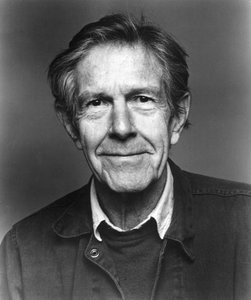
\includegraphics[height=7in]{images/john-cage-portrait.jpg}

  {\small WikiArt.org CC-BY }
\end{center}

\newpage

%%%%% Donald Gillies

\begin{center}
  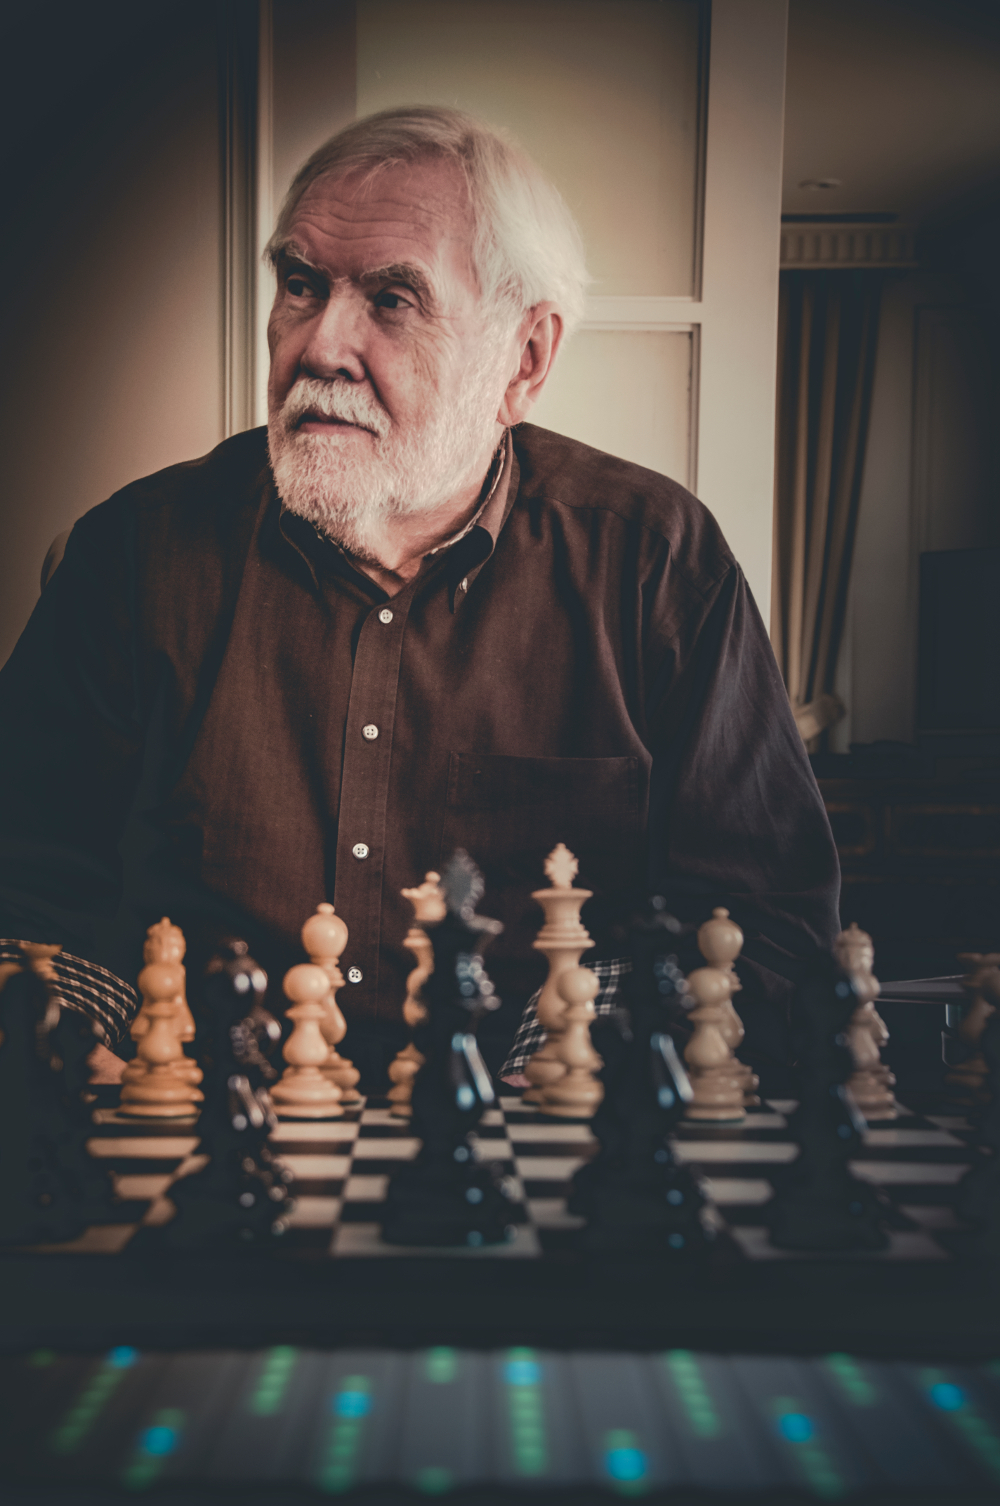
\includegraphics[height=7in]{images/blakeney-gillies-029.jpg}

  {\small © William Blakeney 2019 }
\end{center}

\newpage

%%%%% John Cage

\begin{center}
  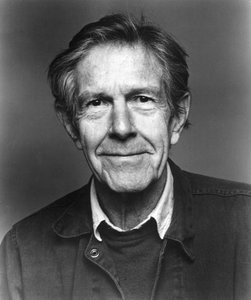
\includegraphics[height=7in]{images/john-cage-portrait.jpg}\\
  {\small WikiArt.org CC-BY }
\end{center}

\newpage

%%%%% 4' 33`' Score

\begin{center}
  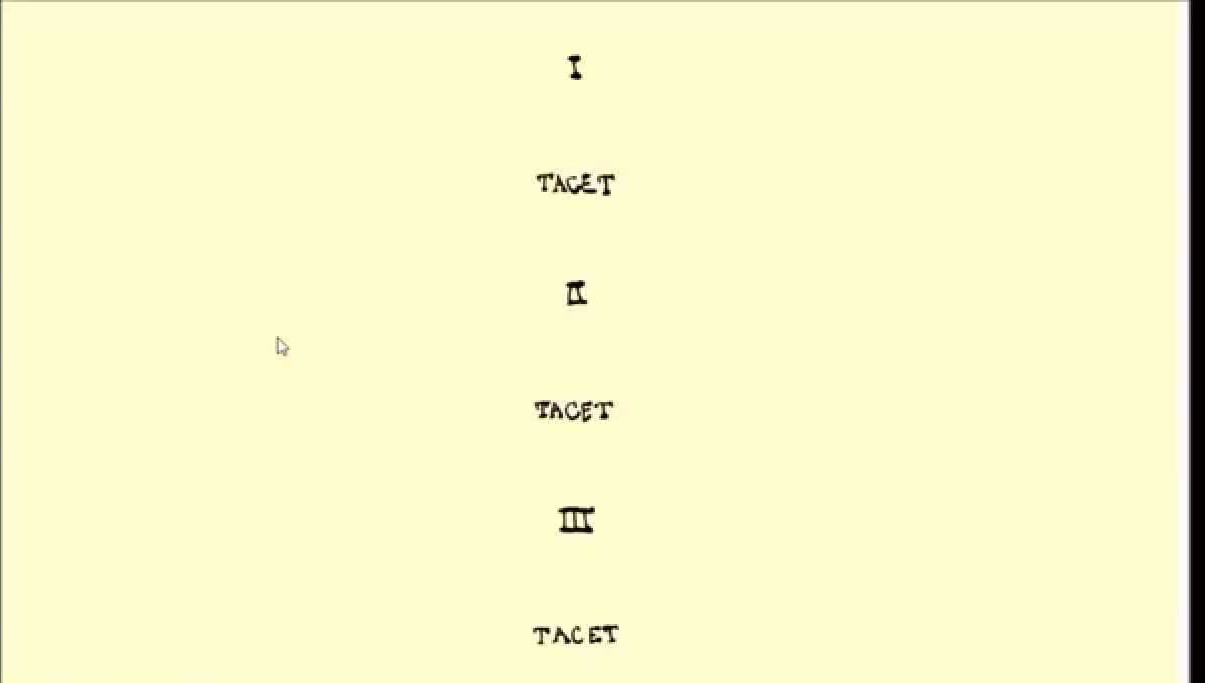
\includegraphics[height=6in]{images/433-score.jpg}
\end{center}

\newpage

%%%%% Authority is constructed and contextual

\vspace*{1in}

{\Huge

\begin{center}

  \resizebox{10in}{!}{\textsc{authority}} \\
  \vspace{1in}
  \resizebox{10in}{!}{\textsc{is constructed}} \\
  \vspace{1in}
  \resizebox{10in}{!}{\textsc{and contextual}}

\end{center}

\newpage

%%%%% Definition of the frame.

{\Huge

  \begin{center}

    Information resources reflect their creators’ expertise and credibility, and are evaluated based on the information need and the context in which the information will be used. Authority is constructed in that various communities may recognize different types of authority. It is contextual in that the information need may help to determine the level of authority required.

\end{center}

}

\newpage

%%%%% Definition of the frame: sentence 1

{\Huge

  \begin{center}

    Information resources reflect their creators’ expertise and credibility, and are evaluated based on the information need and the context in which the information will be used. \textcolor{gray}{Authority is constructed in that various communities may recognize different types of authority. It is contextual in that the information need may help to determine the level of authority required.}

\end{center}

}

\newpage

%%%%% Definition of the frame: sentence 2

{\Huge

  \begin{center}

    \textcolor{gray}{Information resources reflect their creators’ expertise and credibility, and are evaluated based on the information need and the context in which the information will be used}. Authority is constructed in that various communities may recognize different types of authority. \textcolor{gray}{It is contextual in that the information need may help to determine the level of authority required.}

\end{center}

}

\newpage

%%%%% Definition of the frame: sentence 3

{\Huge

  \begin{center}

\textcolor{gray}{Information resources reflect their creators’ expertise and credibility, and are evaluated based on the information need and the context in which the information will be used. Authority is constructed in that various communities may recognize different types of authority.} It is contextual in that the information need may help to determine the level of authority required.

\end{center}

}

\newpage

%%%%% Authority is constructed and contextual.

\vspace*{1in}

{\Huge

\begin{center}

  \resizebox{10in}{!}{\textsc{authority}} \\
  \vspace{1in}
  \resizebox{10in}{!}{\textsc{is constructed}} \\
  \vspace{1in}
  \resizebox{10in}{!}{\textsc{and contextual}}

\end{center}

\newpage

%%%%% John Cage

%% ?? 7in doesn't fit and runs the credit over to the next page??

\begin{center}
  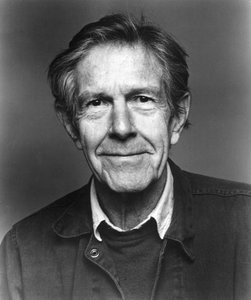
\includegraphics[height=6.9in]{images/john-cage-portrait.jpg}\\
  {\small WikiArt.org CC-BY }
\end{center}

\newpage

%%%%% Entoloma sinuatum

\begin{center}
  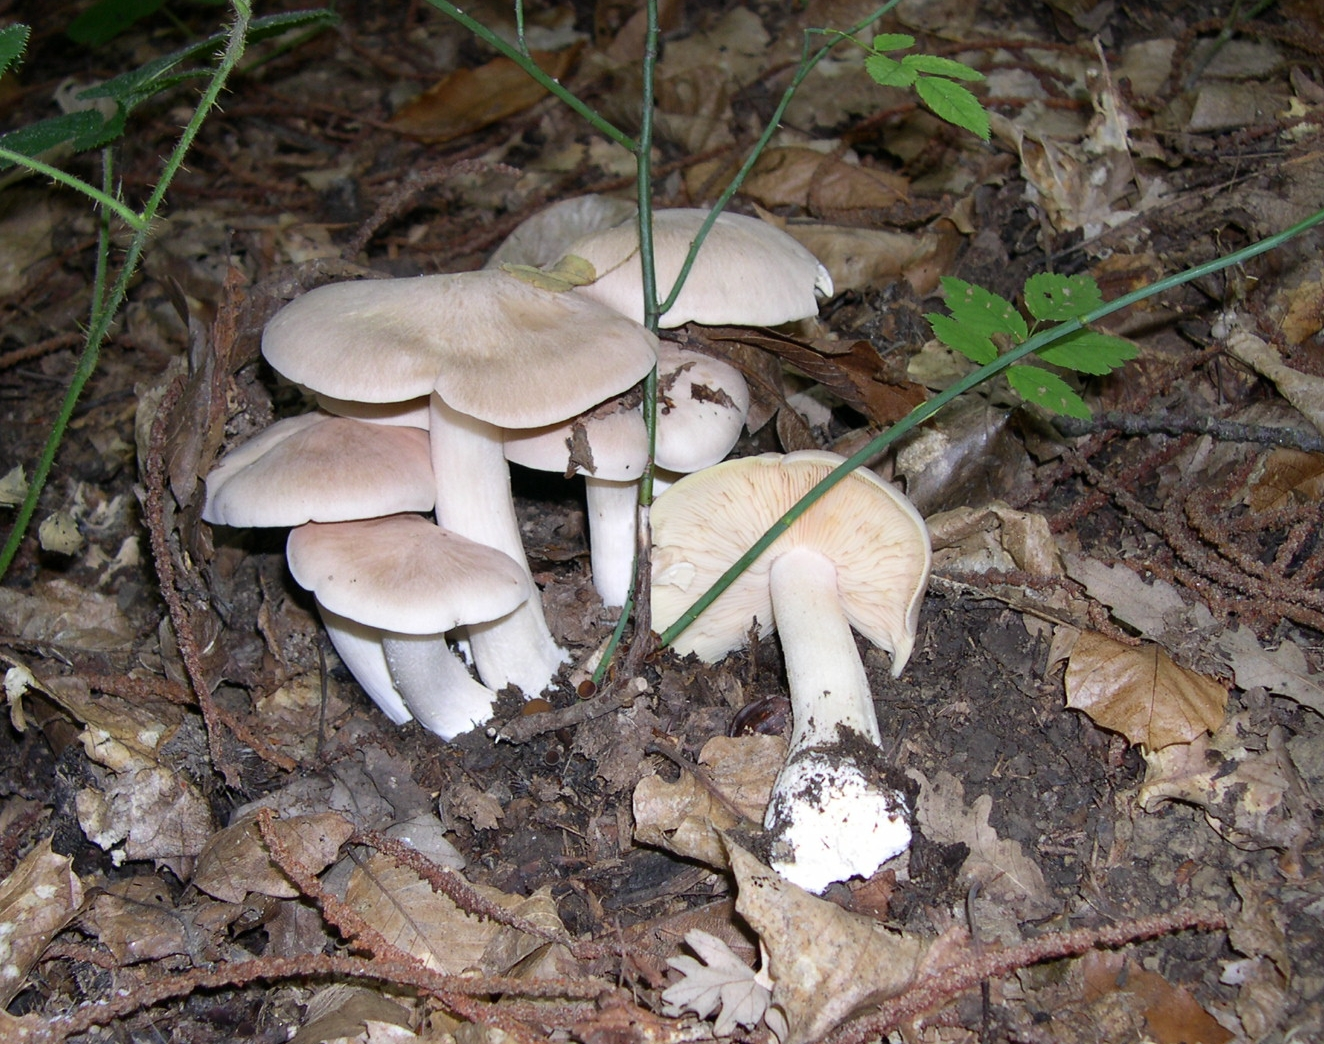
\includegraphics[height=6.5in]{images/entoloma-sinuatum.jpg}

  {\tiny (\textit{Entoloma sinuatum}, Wikipedia CC BY-SA)}
\end{center}

\newpage

%%%%% Definition of the frame.

{\Huge

  \begin{center}

    Information resources reflect their creators’ expertise and credibility, and are evaluated based on the information need and the context in which the information will be used. Authority is constructed in that various communities may recognize different types of authority. It is contextual in that the information need may help to determine the level of authority required.

\end{center}

}

%%%%% Authority is constructed and contextual.

\vspace*{1in}

{\Huge

\begin{center}

  \resizebox{10in}{!}{\textsc{authority}}

  \vspace{1in}

  \resizebox{10in}{!}{\textsc{is constructed}}

  \vspace{1in}

  \resizebox{10in}{!}{\textsc{and contextual}}

\end{center}

\newpage

%%%%% 4' 33`' Score

\begin{center}
  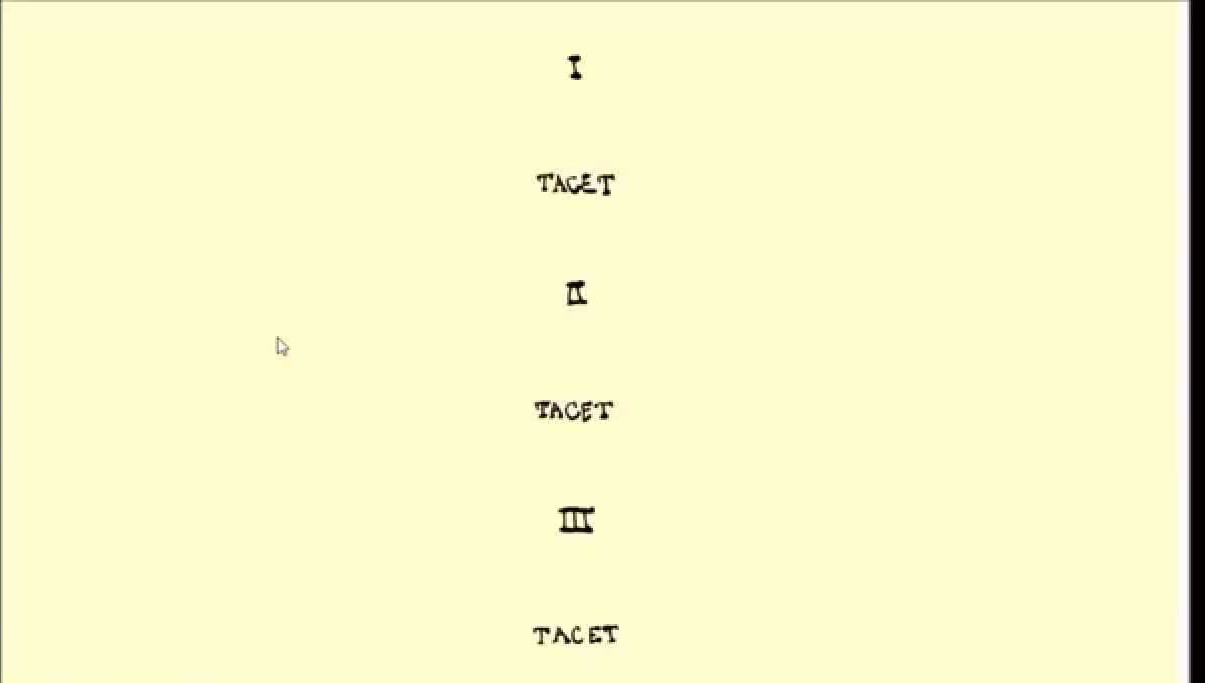
\includegraphics[height=6in]{images/433-score.jpg}
\end{center}

\newpage

%%%%% Theatre Science is constructed and contextual

%%%%% Title

\vspace*{0.5in}

{
  \begin{center}

  \resizebox{10in}{!}{\textsc{theatre}}

  \vspace{0.5in}

  \resizebox{10in}{!}{\textsc{science}}

  \vspace{0.5in}

  \resizebox{10in}{!}{\textsc{is constructed}}

  \vspace{0.5in}

  \resizebox{10in}{!}{\textsc{and contextual}}

\end{center}

}


\end{document}
